% Figure: Clift vs AutoCorres2 comparison
% Using a simple table-based visual since TikZ radar charts are complex
% and pgfplots-based approaches need additional packages
\begin{figure}[t]
\centering
\small
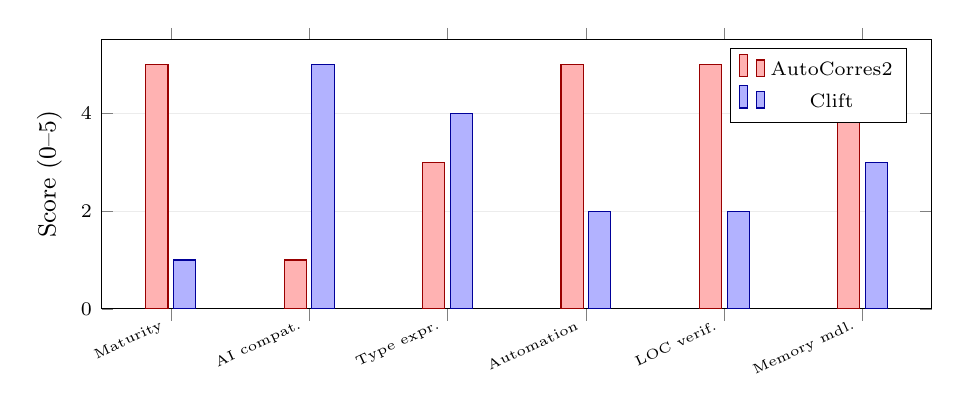
\begin{tikzpicture}
\begin{axis}[
  ybar,
  width=\columnwidth,
  height=5cm,
  bar width=8pt,
  ylabel={Score (0--5)},
  ylabel style={font=\small},
  ymin=0, ymax=5.5,
  xtick=data,
  xticklabels={Maturity, AI compat., Type expr., Automation, LOC verif., Memory mdl.},
  xticklabel style={font=\tiny, rotate=25, anchor=east},
  tick label style={font=\scriptsize},
  legend style={font=\scriptsize, at={(0.97,0.97)}, anchor=north east},
  grid=major,
  grid style={gray!15},
  ymajorgrids=true,
  xmajorgrids=false,
]
% AutoCorres2 scores
\addplot[fill=red!30, draw=red!60!black] coordinates {
  (1, 5) (2, 1) (3, 3) (4, 5) (5, 5) (6, 5)
};
% Clift scores
\addplot[fill=blue!30, draw=blue!60!black] coordinates {
  (1, 1) (2, 5) (3, 4) (4, 2) (5, 2) (6, 3)
};
\legend{AutoCorres2, Clift}
\end{axis}
\end{tikzpicture}
\caption{Qualitative comparison of Clift vs.\ AutoCorres2 across six
axes. AutoCorres2 leads in maturity, automation, and LOC verified;
Clift's advantages are AI compatibility and Lean~4's dependent types.}
\label{fig:radar}
\end{figure}
